\documentclass[11pt]{article}
\pagestyle{plain}
\usepackage[text={6.5in,9.5in},centering]{geometry}
\usepackage{amsmath}
\usepackage{mathrsfs}
\usepackage{parskip}
\usepackage{graphicx}
\usepackage{caption}
\usepackage{float}
\usepackage{xcolor}


\makeatletter
\renewcommand*\env@matrix[1][c]{\hskip -\arraycolsep
  \let\@ifnextchar\new@ifnextchar
  \array{*\c@MaxMatrixCols #1}}
\makeatother

\counterwithin{equation}{enumi}
\begin{document}

\noindent Nathan Burwig \\
Math 87 HW 2 \\
Due 9/21/2022

\hrulefill

\begin{enumerate}
%%%%%%%%%%%%%%%%%%%%%%%%%%%%%%%%%%%%%%%%%%%%%%%%%%%%%%%%%%%%%%%%%%%%%%%
% Problem 1
%%%%%%%%%%%%%%%%%%%%%%%%%%%%%%%%%%%%%%%%%%%%%%%%%%%%%%%%%%%%%%%%%%%%%%%

\item Consider the function $f(x) = e^x - xe^x$
\begin{enumerate}

\item Find the root of $f$

    We can find the root of $f$ rather simply analytically in the following
    way:
    \begin{align*}
        f(x) &= e^x - xe^xi \\
        0 &= e^x - xe^x \\
        xe^x &= e^x \\
        x &= 1
    \end{align*}

\item Test Newton's method, the secant method, and bisection.

    The points we wish to test for each method, the iteration count, and the
    approximation of the root is all given in the below table (along with the
    iteration count). It was done using the SciPy optimization library.

    \begin{center}
        \begin{tabular}{||c | c | c||}
            \hline
            \multicolumn{3}{||c||}{Bisection} \\
            \hline
            Points & Approximation & Iterations \\
            \hline \hline
            
            (0,2)   & 1.0                   & 1  \\
            (-5,5)  & 1.0000000000002274    & 43 \\
            (-10,2) & 0.9999999999995453    & 43 \\
            (-1,2)  & 0.9999999999995453    & 41 \\
            (0,1)   & 1.0                   & 1  \\
            \hline
        \end{tabular}
    \end{center}


    \begin{minipage}[c]{.5\textwidth}
        \begin{tabular}{||c | c | c||}
            \hline
            \multicolumn{3}{||c||}{Newton's Method} \\
            \hline
            Points & Approximation & Iterations \\
            \hline \hline
            
            0.5     & 1.0                   & 7   \\
            2       & 1.0                   & 7   \\
            10      & 1.0                   & 17  \\
            -0.5    & Failed to converge    & 100 \\
            -5      & Failed to converge    & 100 \\
            \hline
        \end{tabular}
    \end{minipage}
    \begin{minipage}[c]{.5\textwidth}
        \begin{tabular}{||c | c | c||}
            \hline
            \multicolumn{3}{||c||}{Secant Method} \\
            \hline
            Points & Approximation & Iterations \\
            \hline \hline
            
            (0,2)   & 1.0                   & 13   \\
            (0,10)  & Result too large      & -    \\
            (-1,2)  & Failed to converge    & 100  \\
            (-5,5)  & Failed to converge    & 100  \\
            (-10,2) & Failed to converge    & 100  \\
            \hline
        \end{tabular}
    \end{minipage}

    There were two types of errors that came up when attempting this. 1)
    "Result too large" or 2) Failed to converge after X iterations. I have
    logged them accordingly, and listed their iteration number where possible.
    I used 100 as the \texttt{maxiter} value.

\item How do inital parameters impact the success in finding the root of the
    three methods?

    It would seem that the inital parameters have quite a large impact on the
    root finding success of each method. Bisection had 0 failures while the
    Secant method failed nearly every attempt at finding the root, despite not
    having particularly different inital parameters. In particular, the
    Newton/Secant method seems to be sensitive to negative numbers
    and large intervals for this function.

    \newpage

\item Sketch a plot of $f$ and eplain why negative initial parameters are not
    successful for some methods.

    We can quickly plot this function using matplotlib to see the following
    plot.

    \begin{figure}[h]
        \centering
        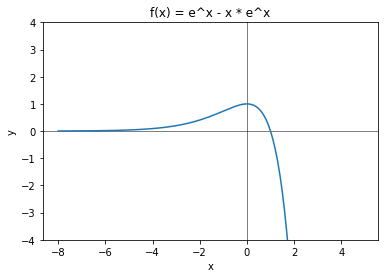
\includegraphics[scale=.6]{output.png}
        \caption{A plot of $f(x)$ }
    \end{figure}

    We can immediately see why we were getting errors for negative numbers and
    larger ranges. as $x \to - \infty$ we see $f(x) \to 0$, thus if the Newton
    or Secant method were given an inital value that was too far into the
    negative $x$, it would iterate too many times, and eventually get close
    enough to 0 as you go out towards infinity (after a very large number of
    iterations of course). This, however, would not be a root.

\item What is a better terminating criteria than $f(x_k) \approx 0$

    We can see from (d) that the termination criteria for the methods should
    not be $f(x_k) \approx 0$ as an asymptote would get arbitrarily close to 0
    without ever reaching it. So we need a more reliable way of determining
    when we are nearing a root. We can consider the slope of our line (secant
    or otherwise) and can attempt to determine based on this. If the slope of
    our line is within some small percentage of difference from the last time,
    we know we are on a shallow slope, and therefore could be on an asymptote.
    If we know that the slope is somewhat steeper than the previous iteration,
    and that we are within an approximation of 0, then it is a safer bet that
    we have actually arrived at a root of the function.

    This is not necessarily always going to work, though. One could imagine a
    line with vanishingly small slope, would eventually satisfy this dual
    condition, even if it wasn't actually at the intercept. I do think, though,
    that it would be a better condition than just $f(x_k) \approx 0$

\end{enumerate}

%%%%%%%%%%%%%%%%%%%%%%%%%%%%%%%%%%%%%%%%%%%%%%%%%%%%%%%%%%%%%%%%%%%%%%%
% Problem 2
%%%%%%%%%%%%%%%%%%%%%%%%%%%%%%%%%%%%%%%%%%%%%%%%%%%%%%%%%%%%%%%%%%%%%%%

\item Consider the optimization problem, max $f(x,y) = x + 2y$ subject to:
\begin{align*}
    y       &\leq 9    \\
    -y      &\leq -1   \\
    2x + y  &\leq 25   \\
    -2x - y &\leq -9   \\
    -2x + y &\leq 1    \\
    2x - y &\leq 15    \\
\end{align*}

\newpage

\begin{enumerate}
    \item Draw the feasible region. Label the boundary curves and corner
        points.

    Using matplotlib, we can create a rough graph of the feasible region (I
    could not figure out how to make the resolution of the imshow image higher,
    so I apologize for it's rather blocky and inaccurate nature.)

    \begin{figure}[h]
        \centering
        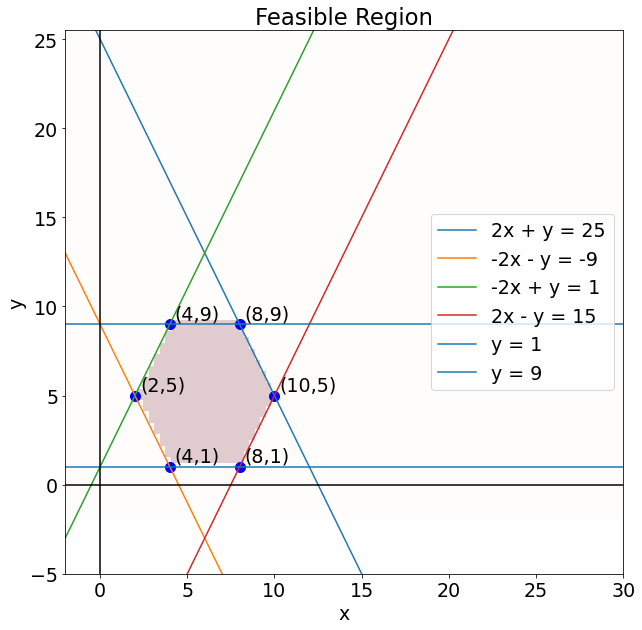
\includegraphics[scale=.4]{feasible.png}
        \caption{A plot of the feasible region of our constraing problem }
    \end{figure}

\item Find the maximum of $f$ and where it occurs.

    We can find the maximal value point by simply testing all the corner points
    in our objective function. Doing so, yields the following results.

    \begin{table}[h]
        \centering
            \begin{tabular}{|| c | c ||}
                \hline
                Points & Values \\
                \hline \hline
                (4,9)   &   22  \\
                (2,5)   &   12  \\
                (8,9)   &   26  \\
                (10,5)  &   20  \\
                (8,1)   &   10  \\
                (4,1)   &   6   \\
                \hline
            \end{tabular}
    \end{table}

    So we can clearly see the maximal value is 26, and it occurs at point
    (8,9).

    \newpage
\item Verify your answer using SciPy.

    We can quickly verify the above answer using SciPy. We can setup a serires
    of arrays that quantify our system. First is the $A$ array which represents
    the coefficients of our constraint inequalities.

    \[
        A =
        \begin{bmatrix}[r]
            0   &   1   \\
            0   &   -1  \\
            2   &   1   \\
            -2  &   -1  \\
            -2  &   1   \\
            2   &   -2  
        \end{bmatrix}, \;\;\;
        b =
        \begin{bmatrix}[r]
            9   \\
            -1  \\
            25  \\
            -9  \\
            1   \\
            15
        \end{bmatrix}, \;\;\;
        c = 
        \begin{bmatrix}
            1  &  2   
        \end{bmatrix}
    \]

    Then we have the matrices b and c. The b matrix are the constraints
    themselves, while the c matrix is based on our objective function. We can
    then solve this using SciPy in the following way:

    \begin{center}
        \begin{verbatim}
            from scipy.optimize import linprog

            A = np.array([[ 0,  1],
                          [ 0, -1],
                          [ 2,  1],
                          [-2, -1],
                          [-2,  1],
                          [ 2, -1]])
            b = np.array([9, -1, 25, -9, 1, 15])
            
            c=np.array([1, 2])
            
            # note the -1 in front of the c as linprog can only 
            # minimize (the same as maximizing the negative)
            res = linprog(-1*c, A_ub=A, b_ub=b)
            print(res)
        \end{verbatim}
    \end{center}

    Running the above code block gives us some output, the important parts
    being:

    \begin{center}
    \begin{verbatim}
            fun: -25.999999999969482
            ...
            x: array([8., 9.])   
    \end{verbatim}
    \end{center}

    Which align exactly with the maximal value and point we found in our table
    seen above (part b).

\end{enumerate}

\newpage

%%%%%%%%%%%%%%%%%%%%%%%%%%%%%%%%%%%%%%%%%%%%%%%%%%%%%%%%%%%%%%%%%%%%%%%
% Problem 3
%%%%%%%%%%%%%%%%%%%%%%%%%%%%%%%%%%%%%%%%%%%%%%%%%%%%%%%%%%%%%%%%%%%%%%%

\item Some very type A bakers

    A bakery wants to sell forty five Valentine’s Day gift bags. They have decided to offer two
    types of bags: Bags of type A will contain four of cupcakes and two cookies, and bags of
    type B will contain two cupcakes and five cookies. Baskets of type A will
    be sold for \$12 and baskets of type B will be sold for \$16. The bakery has 
    90 cookies and 115 cupcakes in total.
    
    \begin{enumerate}
        \item Solve for how many baskets of each type should be made to
            maximize the profits of the bakery. If it is fractional, round down
            to the nearest whole number solution.

        We can start, by ordering our system in a table according to the types
        of baskets, and the quantity of each item within those baskets.

        \begin{center}
            \begin{tabular}{|| c || c | c ||}
                \hline
                            & Cupcakes (c)  &   Cookies (k) \\
                \hline \hline
                Basket A    & 4             &   2   \\
                \hline
                Basket B    & 2             &   5   \\
                \hline
                Total       & 115           &   90  \\
                \hline
            \end{tabular}
        \end{center}

        With this, we can quickly setup our optimization innequalities, but
        first, we should figure out our objective function. It should take the
        following form...
        \[P(a,b) = 12a + 16b\]
        Now we can list our constraints based on the table above...
        \begin{align*}
            4a + 2b &\leq 115   \\
            2a + 5b &\leq 90    \\
        \end{align*}
        We also know that (of course) $c \geq 0$ and $k \geq 0$

        Given the following information, we can either draw the feasible region
        and solve, or we can construct arrays to use SciPy linprog again. I
        will do the latter method, to save time and space. 

        Then we have the following matrices...

        \[
            A = 
            \begin{bmatrix}[r]
                4   &   2   \\
                2   &   5   \\
            \end{bmatrix}, \;\;\;
            b = 
            \begin{bmatrix}[r] 
                115 \\
                90  
            \end{bmatrix}, \;\;\;
            c = 
            \begin{bmatrix}[r]
                12 & 16                
            \end{bmatrix}
        \]

        Which we can plug into SciPy in the exact same way as seen in 2.c to
        get the following result.

        
            \begin{center}
            \begin{verbatim}
                fun: -426.2499990846053
                ...
                x: array([24.68749995,  8.12499998])
            \end{verbatim}
            \end{center}

        Thus, we have our maximal value at (24, 8) or 24 of type A baskets and
        8 type B baskets, which, upon plugging into our objective function,
        returns the maximal profit or \$416.

        One can double check this result, by quickly plotting the constraint
        function on an application like desmos, and can see that this is, in
        fact, the optimal value.


    \end{enumerate}
    

    

\end{enumerate}
\end{document}
